%  Arrange the long version by Chen, August 2, 2001
%
%  Minor corrections by L'Ecuyer, December 20, 2001
%  Rewritten (shorter  version) by L'Ecuyer, July 5, 2001
%  Touched by Kelton, December 18, 2000
%  Touched by L'Ecuyer, December 8, 2000
%  Touched by Simard,   December 6, 2000

\documentclass[12pt]{article}
% \usepackage{secdot}
\usepackage{epsfig}
\usepackage{url}
%\usepackage{amsfonts}

\newif\iflong\longfalse
\longtrue         %  Put to true to obtain longer version.
\newenvironment{longversion}{\iflong}{\fi}

\marginparwidth 0pt\marginparsep 0pt \topskip 0pt\headsep
0pt\headheight 0pt \oddsidemargin 0pt\evensidemargin 0pt\textwidth
6.5in \topmargin 0.0in\textheight 9.0in

\newcommand{\singlespace}{\baselineskip 13.60pt plus .3pt minus .1pt}
\newcommand{\sesquispace}{\baselineskip 20.40pt plus .3pt minus .1pt}
\newcommand{\doublespace}{\baselineskip 27.20pt plus .3pt minus .1pt}

\newenvironment{hangproc}{\begin{list}{}{\setlength{\itemsep}{0pt}
               \setlength{\parsep}{0pt} \setlength{\leftmargin}{+\parindent}
               \setlength{\itemindent}{-\parindent}}}{\end{list}}

\newenvironment{hangref}{\begin{list}{}{\setlength{\itemsep}{4pt}
               \setlength{\parsep}{0pt}\setlength{\leftmargin}{+0.25in}
               \setlength{\itemindent}{-0.25in}}}{\end{list}}

\catcode`\@=11  %%%%%%%%%%%

% For the bibliography.

\newenvironment {refer}{
  \begin {list}{}{
  \def\newblock {\hskip .11em plus .33em minus .07em}
  \setlength {\itemsep}{2pt}
  \setlength {\parsep}{0pt}
  \setlength {\parindent}{20pt}
  \setlength {\leftmargin}{+\parindent}
  \setlength {\itemindent}{-\parindent}}}{\end{list}}
\def\@biblabel#1{}

%\def\cite{\@ifnextchar [{\@tempswatrue\@citex}{\@tempswafalse\@citex[]}}

\def\citeN{\@ifnextchar [{\@tempswatrue\@citexp}{\@tempswafalse\@citexp[]}}

\def\@cite#1#2{\null{#1\if@tempswa , #2\fi}\relax }

\def\@citex[#1]#2{\if@filesw\immediate\write\@auxout{\string\citation{#2}}\fi
  \def\@citea{}\@cite{\@for\@citeb:=#2\do
    {\@citea\def\@citea{, }\@ifundefined
       {b@\@citeb}{{\bf ?}\@warning
       {Citation `\@citeb' on page \thepage \space undefined}}%
  {\csname b@\@citeb\endcsname}}}{#1}}

\def\@citexp[#1]#2{\if@filesw\immediate\write\@auxout{\string\citation{#2}}\fi
  \def\@citea{}\@cite{\@for\@citeb:=#2\do
    {\@citea\def\@citea{, }\@ifundefined
       {p@\@citeb}{{\bf ?}\@warning
       {Citation `\@citeb' on page \thepage \space undefined}}%
  {\csname p@\@citeb\endcsname}}}{#1}}

\def\bibcite#1#2#3{\global\@namedef{b@#1}{#2\ #3}}

\def\bibciteN#1#2#3{\global\@namedef{p@#1}{#2\ (#3)}}

\def\@lbibitem[#1][#2]#3{\item[\@biblabel{#1}]\if@filesw
        { \def\protect##1{\string##1\space}
          \immediate\write\@auxout{\string\bibcite{#3}{#1}{#2}}
          \immediate\write\@auxout{\string\bibciteN{#3}{#1}{#2}}
          \fi\ignorespaces}}

%% Sections, figures, tables.

\newfont{\sfbold}{cmssbx10 scaled 1000}
\def\section{\@startsection {section}{1}{\z@}{-2.5ex plus -1ex minus
 -.2ex}{2.3ex plus .2ex}{\sfbold}}
\def\subsection{\@startsection{subsection}{2}{\z@}{-2.25ex plus -1ex minus
 -.2ex}{1.0ex plus .2ex}{\sfbold}}

%\def\thesection       {\arabic{section}.}
%\def\thesubsection    {\thesection\arabic{subsection}.}
\long\def\@makecaption#1#2{
 \vskip 10pt
 \hbox to \hsize{\hfil #1\hfil}
 \setbox\@tempboxa\hbox{#2}
 \ifdim \wd\@tempboxa >\hsize \unhbox\@tempboxa\par \else
   \hbox to\hsize{\hfil\box\@tempboxa\hfil}
 \fi}
\def\fnum@table{{\bf Table~\Roman{table}}}
\def\fnum@figure{{\bf Figure~\arabic{figure}}}
\renewcommand{\thetable}{\Roman{table}}
\renewcommand{\thefigure}{\arabic{figure}}

\catcode`\@=12  %%%%%%%%%

% Macros pour inserer des bouts de code (programmes).
% Faire  \code ...  \endcode
{\obeyspaces\gdef {\ }}
\def\setverbatim{\def\par{\leavevmode\endgraf}
            \parskip=0pt\parindent=0pt\obeylines\obeyspaces }
\chardef\other=12
\def\ttverbatim{\setverbatim\tt
       \catcode`\{=\other \catcode`\}=\other \catcode`\_=\other
       \catcode`\^=\other \catcode`\$=\other \catcode`\%=\other
       \catcode`\#=\other \catcode`\&=\other \baselineskip=11pt
       }  %$
    % Reproduit tel quel ce qui est ecrit, en caracteres \tt.
    % On doit faire  \begingroup\ttverbatim   ....  \endgroup
\def\code {\vfil\vfilneg\vbox\bgroup\ttverbatim}
\def\longcode {\vfil\vfilneg\bgroup\ttverbatim}
\def\smallc {\small\tt\baselineskip=9.5pt}
\let\endcode=\egroup
\def\parup{\nobreak\vskip -2pt\nobreak}
\def\tab{\small\parindent=0pt\advance\leftskip by 1.5em\parup}
\def\tabb{\small\parindent=0pt\advance\leftskip by 3.0em\parup}
\def\endtab{\vskip 0.01pt\advance\leftskip by -1.5em\normalsize}
\def\endtabb{\vskip 0.01pt\advance\leftskip by -3.0em\normalsize}
%
\def\hide{\iffalse}
\let\endhide=\fi

%\newcommand{\ZZ}{{\mathbb{Z}}}
\newcommand{\ZZ}{{\bf Z}}

%%%%%%%%%%%%%%%%%%%%%%%%%%%%%%%%%%%%%%%%%%%%%%%%%%%%%%%%%%%%%%%
\begin{document}

\begin{center}
{\Large\sfbold AN OBJECT-ORIENTED RANDOM-NUMBER PACKAGE
 WITH MANY LONG STREAMS AND SUBSTREAMS}

\bigskip

{\sfbold PIERRE L'ECUYER and RICHARD SIMARD}\\
{\small\it D\'{e}partement d'informatique et de recherche
op\'{e}rationnelle, Universit\'{e} de Montr\'{e}al, C.P.\
6128 succ.\ Centre-Ville, Montr\'{e}al, Qu\'{e}bec H3C 3J7,
Canada\\ lecuyer@iro.umontreal.ca $\bullet$ simardr@iro.umontreal.ca}

\bigskip

{\sfbold E.\ JACK CHEN}\\
{\small\it BASF Corporation, 3000 Continental Drive--North,
Mount Olive, New Jersey 07828--1234, USA\\ chenej@basf.com}

\bigskip

{\sfbold W. DAVID KELTON}\\
{\small\it Department of Management Science and Information Systems,
The Smeal College of Business Administration, 303 Beam,
The Pennsylvania State University, University Park, PA 16802-1913, USA \\
dkelton@psu.edu}

\bigskip

(Received December 2000)

\end{center}

\medskip

\noindent
Multiple independent streams of random numbers are often required
in simulation studies, for instance, to facilitate synchronization
for variance-reduction purposes, and for making independent
replications.  A portable set of software utilities is described
for uniform random-number generation. It provides for multiple
generators (streams) running simultaneously, and each generator
(stream) has its sequence of numbers partitioned into many long
disjoint contiguous substreams.
The basic underlying generator for this implementation is a combined
multiple recursive generator with period length of
approximately $2^{191}$, proposed in a previous paper.
% $(\approx 3.1\times 10^{57})$, good speed,
% and excellent theoretical properties.
A C++ interface is described here. Portable implementations are
available in C, C++, and Java via the On-line Companion to this %wdk
paper on the {\it Operations Research\/} website. %wdk
% Simple procedure calls allow the
% user to make any generator ``jump'' ahead/back $v$ steps (random
% numbers). Implementation issues are discussed. An efficient and
% portable code is also provided to implement the package.

\iflong %%%
This report is an expanded version of the article by \citeN{rLEC01s}.
\fi  %%%

\bigskip

\noindent {\it Subject classifications:} Simulation: Random number generation,
Simulation: Random variable generation, Simulation: Statistical analysis,
Computers/computer science: Software

\bigskip\hrule\bigskip

\sesquispace

%%%%%%%%%%%%%%%%%%%%%%%%%%%%%%%%%%%%%%%%%%%%%%%%%%%%%%%%%%%%%%%%
% \section {INTRODUCTION}

\noindent
Experts now recognize that small linear
congruential generators (LCGs) with moduli
around $2^{31}$ or so should no longer be used as general-purpose
random-number generators (RNGs). Not only can one exhaust the
period in a few minutes on a PC, but more importantly the poor
structure of the points can dramatically bias simulation results
for sample sizes much smaller than the period length.

\iflong %%%%%%%  For long version only.  Perhaps just remove?
As an illustration, we consider a variant of the {\em birthday\/}
problem, defined as follows. Partition the unit square $[0,1)^2$
into $k$ cells (square boxes) of equal sizes. Identify these cells
as $0$ through $k-1$. If we generate $2n$ random numbers
$U_0,\dots,U_{2n-1}$, then each non-overlapping 2-tuple $V_{i} =
(U_{2i},U_{2i+1})$, $i=0,\dots,n-1$, will fall into some cell $I_i
\in \{0, \dots, k-1\}$. Let $I_{(1)}\le I_{(2)} \le \cdots \le
I_{(n)}$ be the identification of the cells sorted by increasing
order. Compute the {\em spacings\/} $S_j = I_{(j+1)}-I_{(j)}$, for
$j=1,\dots,n-1$, and let $Y$ be the number of values of $j \in
\{1,\dots,n-2\}$ such that $S_{(j+1)} = S_{(j)}$, where
$S_{(1)},\dots,S_{(n-1)}$ are the spacings sorted by increasing
order. These $n$ cells can be viewed as the birthdays (between day
0 and day $k-1$) of $n$ people in a world where years have
$k$ days, whence the name {\em birthday spacings\/}
(\cite{rMAR85a,rLEC01a}).
% (Marsaglia 1985; L'Ecuyer and Simard 2000).
Suppose we want to estimate $E[Y]$
by simulation, using the LCG:
 $$ x_i = a x_{i-1} \bmod m, \quad u_i = x_i/m,\quad
    x_0\in\{1,\dots,m-1\}, $$
with $a = 16807$ and $m = 2^{31}-1$.
This LCG is widely used. We made ten replications of the
simulation, with $n = 2^{15} = 32768$ and $k \approx 2^{43}$, and
obtained ten values of $Y$ ranging from 1315 to 1404. (Each
replication takes $< 0.02$ sec on a PC.) One may then conclude
that $E[Y]$ is somewhere between 1300 and 1400. In fact, it can be
shown (theoretically) that $Y$ has approximately the Poisson
distribution with mean $\lambda = n^3/(4k)$ when $n$ is large and
$\lambda$ is small (\cite{rMAR85a}). Here, we took $k \approx
n^3/4$, so $E[Y] = \lambda\approx 1$. The above estimate is thus
very far from the truth! If $Y$ takes the value $y$, the (right)
$p$-value is $p^+(y) = P[Y\ge y\mid H_0]$, where $H_0$ is the null
hypothesis that $E(Y)=y$. Table~\ref{birthday} gives the estimated
value $y$ of $E(Y)$, and the corresponding $p$-value, with
different values of $n$ and with $k\approx n^3/4$. In all cases,
the true distribution of $Y$ is approximately Poisson with mean 1.
For $n \ge 2^{13}$, the $p$-values are virtually zero, i.e., the
estimates are highly inaccurate. Changing the multiplier $a$
brings no significant improvement: All LCGs start to fail at $n
\approx 8 m^{1/3}$. The problem is that the structure of the
points is much too regular.
We clearly need better RNGs!
%Other limitations of LCGs in statistical tests are discussed, e.g.,
%by \citeN{rENT98a,rHEL95a,rHEL98a,rLEC98h}.

\begin {table}
\caption {$p$-values for the birthday problem.} \label{birthday}
\renewcommand {\arraystretch}{0.85}
\begin {center}
\begin {tabular}{ccc}
\hline
  $n$     &  $y$  &  $p^+(y)$  \\
\hline
 &&\\
 $2^{12}$ &     2 & 0.26  \\
 $2^{13}$ &    16 & $1.9\times 10^{-14}$ \\
 $2^{14}$ &   170 & $ < 10^{-15}$  \\
 $2^{15}$ &  1310 & $ < 10^{-15}$  \\
 $2^{16}$ & 10060 & $ < 10^{-15}$  \\
 $2^{17}$ & 53907 & $ < 10^{-15}$  \\ \hline
\end {tabular}
\end {center}
\end{table}

%
\else  %%%%%  (for short version)
%
As an example, \citeN{rLEC01a}  % L'Ecuyer and Simard (2001)
consider a simple simulation problem where $n$ points are generated
randomly in $k$ cells over the two-dimensional square, to estimate the
expected number of {\em repeated\/} values for the spacings between
successive cells that contain a point.
They find that with a LCG of the form
$$
  x_i = a x_{i-1} \bmod m, \quad u_i = x_i/m,\quad
        x_0\in\{1,\dots,m-1\},
$$
if $k$ is large ($\approx n^3/4$) and $n\approx 8 m^{1/3}$ (or
more), the simulation gives totally wrong results, regardless of
$m$ and $a$. This means only $n \approx 10,000$ for $m\approx %wdk
2^{31}$ and $n \approx 500,000$ for $m\approx 2^{48}$. %wdk
\fi  %%%%%%%%%%%

%--- Better RNGs proposed.
Much better RNGs have already been proposed to replace older %wdk
unsafe LCGs.  We mention, for instance, the Mersenne twister of
\citeN{rMAT98a}, the combined MRGs of \citeN{rLEC99b}, the
combined LCGs of \citeN{rLEC97d}, and the combined Tausworthe
generators of \citeN{rLEC99a}. All of these have fairly solid
theoretical support, have been extensively tested, and are easy to
use.

%--- Need for multiple streams.
However, a single RNG does not always suffice.
Many disjoint random-number subsequences, each having long period
and good statistical properties, are often required in simulation
studies, for instance, to make independent replications or to
associate distinct ``streams'' of random numbers with different
sources of randomness in the system to facilitate synchronization
for variance reduction (\cite{sLAW00a}).
\iflong  %%%%%%
Suppose, for instance, that one wants to
perform independent pairs of replications with common random
numbers across the configurations (i.e., between any two
replications of the same pair) in order to compare two different
competing configurations of a system. To ensure proper
synchronization, we want every generator to start from the same
seed in both runs of the same pair. However, in general, these two
runs will make a different number of calls to a generator, and
programming ``tricks'' have to be used to skip a proper amount of
random numbers to resynchronize the generators for the next pair
without overlap in the random-number streams. This requires extra
programming effort and is error-prone. Good software tools
should ease the programmer's task in that respect (\cite{rLEC91a}).
% L'Ecuyer and C\^{o}t\'{e} 1991).
\fi  %%%%%%%

In this paper, we propose a package for uniform random-number
generation with multiple streams of (pseudo)random numbers and
convenient tools to move around within and across these streams.
The structure and the tools offered are similar to those in the
package proposed by \citeN{rLEC91a} and \citeN{rLEC97d}.
% L'Ecuyer and C\^{o}t\'{e} (1991) and L'Ecuyer and Andres (1997).
The main differences are:

\begin{itemize}
%
\item
The underlying ``backbone'' generator is
more robust and has longer period than those used by these authors.
% in L'Ecuyer and C\^{o}t\'{e} (1991) and L'Ecuyer and Andres (1997).
We use the {\em combined multiple recursive generator\/} (CMRG)
{\tt MRG32k3a} proposed by \citeN{rLEC99b}.  %%  L'Ecuyer (1999).
% Its period length is near $2^{191}$ and its state can be represented
% over 192 bits.
% (\approx 3.1 \times 10^{57})$ and
% and excellent statistical properties.

\item
The package proposed here has an object-oriented design.
The {\em streams}, which can be seen as virtual RNGs,
are declared at will, as instances of a {\em class},
instead of being numbered from $0$ to $N$ where $N$ is fixed.
% Each stream of random numbers is an object of the class {\tt RngStream}.

\iflong  %%%%
\item
The generator is implemented in floating-point arithmetic
instead of integer arithmetic.
This is faster on most current 32-bit computers, for which 64-bit
floating-point operations are implemented in hardware on the CPU.
%
\fi  %%%%
\end{itemize}


%--- Other multiple streams packages...: Mascagni.
Other random number packages with multiple streams have been proposed
in recent years;  see for example \citeN{rMAS00a}.
% -- also GNU, Java, ...
These packages do not offer the same tools for streams and
substreams as ours, and are not supported by the same
theoretical analysis for the quality and independence
of the different streams.
%  In fact: analysis is weak or simply absent.

%--- Overview of the paper.
% \subsection {Overview of the Paper}

\iflong  %%%%%%%%%%%

The rest of this paper is organized as follows.
Section \ref {sec:description}
provides some background on the backbone CMRG and explains the idea
of multiple streams and substreams.
In Section \ref {utility}, we describe support utilities.
We give a quick and easy way to compute $a \times s \bmod m$
for any positive integer values of $a<m$, $s<m$, and $m<2^{32}$,
for computers that support the IEEE-754 standard
(which ensures that floating-point numbers have at least
53 bits of precision for the mantissa).
We also describe a code to compute $A^{v} \bmod m$, where $A$ is
a square matrix of integers.
These kinds of computations are required for jumping by several
steps at a time in the generator's sequence
(e.g., for jumping to distant streams or substreams).
Section \ref{RNG} describes a package with
multiple streams and substreams,
%, and can be read independently of Sections \ref {sec:description}
% \ref{backbone}
% and \ref{utility}.
and gives the interface of its C++ implementation.
Section \ref{example} provides
some examples of using this RNG package.
Section \ref{summary} summarizes.
The appendix gives the complete C++ implementation.
Implementations in C and Java are available
% from the authors.
at \url{http://www.iro.umontreal.ca/~lecuyer}.

\else  %%%%%%%%%  (short version)

In what follows, we provide some background on the backbone CMRG,
explain how the streams and substreams are defined,
and give a C++ interface to the package.
Implementations in C, C++, and Java, as well as a more detailed version
of this paper, are available
% from the authors.
in the Online Companion to this paper on the {\it Operations %wdk
Research\/} website, and at \url{http://www.iro.umontreal.ca/~lecuyer}. %wdk

\fi  %%%%%%%%%%


%%%%%%%%%%%%%%%%%%%%%%%%%%%%
\section {DESCRIPTION AND IMPLEMENTATION OF THE SOFTWARE}
\label {sec:description}

\subsection {The underlying backbone generator}
\label {backbone}

\citeN{rLEC99b}  % L'Ecuyer (1999)
gave several good parameter sets for CMRGs of
different sizes.  We have selected one of them,
called {\tt MRG32k3a}, as our backbone generator.
It has 2 components each of order 3.
At step $n$, its state is the pair of vectors
$s_{1,n}=(x_{1,n},x_{1,n+1},x_{1,n+2})$ and
$s_{2,n}=(x_{2,n},x_{2,n+1},x_{2,n+2})$, which evolve according to
the linear recurrences
\begin{eqnarray*}
 x_{1,n} & = & (1403580\times x_{1,n-2}-810728\times x_{1,n-3}) \bmod m_1 \\
 x_{2,n} & = & (527612\times x_{2,n-1}-1370589\times x_{2,n-3}) \bmod m_2,
\end{eqnarray*}
where $m_{1}=2^{32}-209 = 4294967087$ and $m_{2}=2^{32}-22853 = 4294944443$,
and its output $u_n$ is defined by
\begin{eqnarray*}
 z_{n}  & = & (x_{1,n}-x_{2,n}) \bmod 4294967087 \\
 u_n    & = & \left \{
 \begin{array}{lll}
  & z_n / 4294967088 & \mbox{   if } z_n > 0 \\
  & 4294967087 / 4294967088 & \mbox{   if } z_n = 0.
 \end{array}
\right.
\end{eqnarray*}
Its period length is $\rho = (m_{1}^{3}-1)(m_{2}^{3}-1)/2 \approx
2^{191} \approx 3.1\times 10^{57}$.
RNGs with much longer periods are also available,
but their states must contain more bits and are therefore more expensive
to manipulate.  We think that our choice is a reasonable compromise.
The parameters have been chosen so that the period is
long, a fast implementation is available (in floating point arithmetic),
and the generator performs well with respect to the spectral test in
up to (at least) 45 dimensions.
The spectral test in $t$ dimensions measures the uniformity
of the point set
$$
  T_t = \{(u_0, \ldots, u_{t-1})\ |
    (x_{1,0}, x_{1,1},x_{1,2}) \in \ZZ^3_{m_1},
    (x_{2,0}, x_{2,1},x_{2,2}) \in \ZZ^3_{m_2}\},
$$
where $\ZZ_m = \{0,\dots,m-1 \}$, and makes sure that this set covers
the $t$-dimensional unit hypercube very uniformly.
This $T_t$ is the set of all overlapping $t$-tuples of successive values
produced by the generator, from all possible initial states.
\iflong %%%%
It turns out to be the intersection of a lattice with the $t$-dimensional
unit hypercube.  This means that all the points of $T_t$ lie in a
limited number of equidistant parallel hyperplanes.
The parameters of the generator were chosen so that the distance between the
successive hyperplanes is close to the minimal achievable
distance given the total number of points $m_1 m_2$, for all $t$ up
to 45.
\fi  %%%%

\iffalse  %%%%
%\iflong
Thus, the moduli and coefficients of the recurrences are
$m_{1}=2^{32}-209 = 4294967087$, $a_{11}=0$, $a_{12}=1403580$,
$a_{13}=-810728$, $m_{2}=2^{32}-22853 = 4294944443$,
$a_{21}=527612,a_{22}=0$, and $a_{23}=-1370589$.
This implementation sets $\delta _{1}$ $=-\delta_{2}=1$.
Its coefficients satisfy the
condition that $\ a_{ij}(m_{j}-1) < 2^{53}$, so that the recurrence
has a fast implementation in floating point arithmetic.


\fi  %%%%%


%%%%%%%%%%%%
\subsection {Multiple streams and substreams}

Let $\rho$ be the period length of the RNG and $T$ its
transition function; that is, $T(s_{n}) = s_{n+1}$ where $s_n$
is the generator's state at step $n$, and $T^\rho(s) = s$.
To partition the generator's sequence into disjoint streams and substreams,
we choose two positive integers $v$ and $w$, and let $z=v+w$.
We first cut the long cycle
into adjacent {\em streams\/} of length $Z = 2^z$ and then
partition each of these streams into $V= 2^v$ {\em blocks\/} (or
{\em substreams\/}) of length $W=2^w$.

If $s_0$ is the initial seed of the generator and $I_{g}$ denotes the
{\em initial state\/} of stream $g$ for $g\ge 1$, then we have
$I_1 = s_0$, $I_2 = T^Z(s_0)$, \dots, $I_g = T^Z(I_{g-1}) = T^{(g-1)Z}(s_0),
\dots$.
The first {\em substream\/} of stream $g$ starts in state $I_g$,
the second one in state $T^W(I_g)$, the third one in state $T^{2W}(I_g)$,
and so on.
At any moment during program execution, stream $g$ is in some state, say
$C_{g}$.  We denote by $B_g$ the starting state of the substream that
contains the current state, i.e., of the {\em current substream},
and $N_g = T^W(B_g)$ the starting state of the {\em next substream\/}.
% In Figure~\ref{state1},
In the following illustration, for example, the state of stream $g$ is at
% illustrates an example of a stream whose state is at
the $6^{th}$ value of the third substream, i.e., $2W+5$ steps
ahead of its initial state $I_g$ and 5 steps ahead of $B_g$.
\iflong %%%
Figure~\ref{streams} depicts the overall
arrangement of the streams and substreams, and indicates the
spacings and number of each.
\fi %%%
% \begin{figure}
% \caption {Example of a stream state.}                     \label{state1}
\begin{center}
\def\tick#1{\vrule height 0pt depth #1pt}
\def\enskip{\hskip.5em\relax}
\def\ld{\hbox to 0.24 in{\vtop{\kern3.0pt\hbox{\dotfill}}}}
\def\ts{\enskip\tick4}
\def\suba{\hbox to 1.2in {\vtop
 {\hbox to 1.2in{\hbox to .66in{\hrulefill}\hbox to .30in{\dotfill}\hrulefill}
  \hbox to 1.2in{\tick9\ts\ts\ts\ts\ts\ts\ts\hfill\ts\enskip}}}}
\def\subb{\hbox to 1.2in {\vtop
 {\hbox to 1.2in{\hbox to .84in {\hrulefill}
         \hbox to .24in {\dotfill}\hbox to .12in {\hrulefill}}
  \hbox to 1.2in{\tick9\ts\ts\ts\ts\ts\ts\ts\ts\hfill\ts\enskip}}}}

$$\vbox{\offinterlineskip \hbox to 6.0in{\hskip 2.65in \hbox to
%\vbox{\offinterlineskip \hbox to 6.0in{\hskip 2.4in \hbox to
1.2in{\hfil\hskip1.07em $C_g$\hfil}\hfill} \vskip .1pt \hbox to
6.0in{\hskip 2.65in \hbox to 1.2in{\hfil\hskip1.07em
$\Downarrow$\hfil}
    \hfill}
\vtop {\offinterlineskip\hskip 0.0in \hbox to 5.5 true in
       {\suba\suba\subb\suba\tick9
        \hbox to .12in {\hrulefill}\hbox to .24in{\dotfill}}}\vskip .1pt
%\hskip -0.65in\hbox to 1.2 in{\hfil$I_g$\hfil}\hskip 1.25in
\hskip -1.90in\hbox to 1.2 in{\hfil$I_g$\hfil}\hskip 1.25in
  \hbox to 1.2 in{\hfil$B_g$\hfil}\hbox to 1.2 in{\hfil$N_g$\hfil}\hfill
\vskip .1pt } $$
\end{center}
% \end{figure}

\iflong %%%%
\begin{figure}
\caption {Overall arrangement
   of streams and substreams for the package.}   \label{streams}
\bigskip
\hfil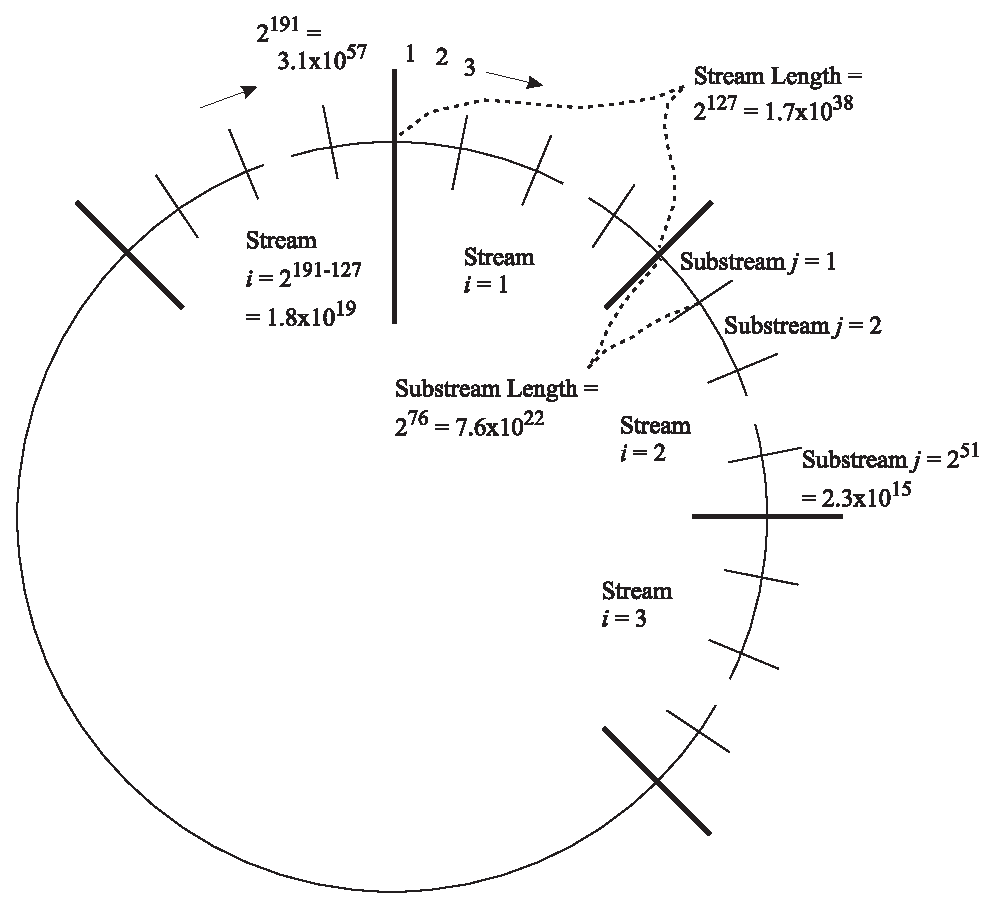
\includegraphics{fig2.eps}\hfil
%\centerline{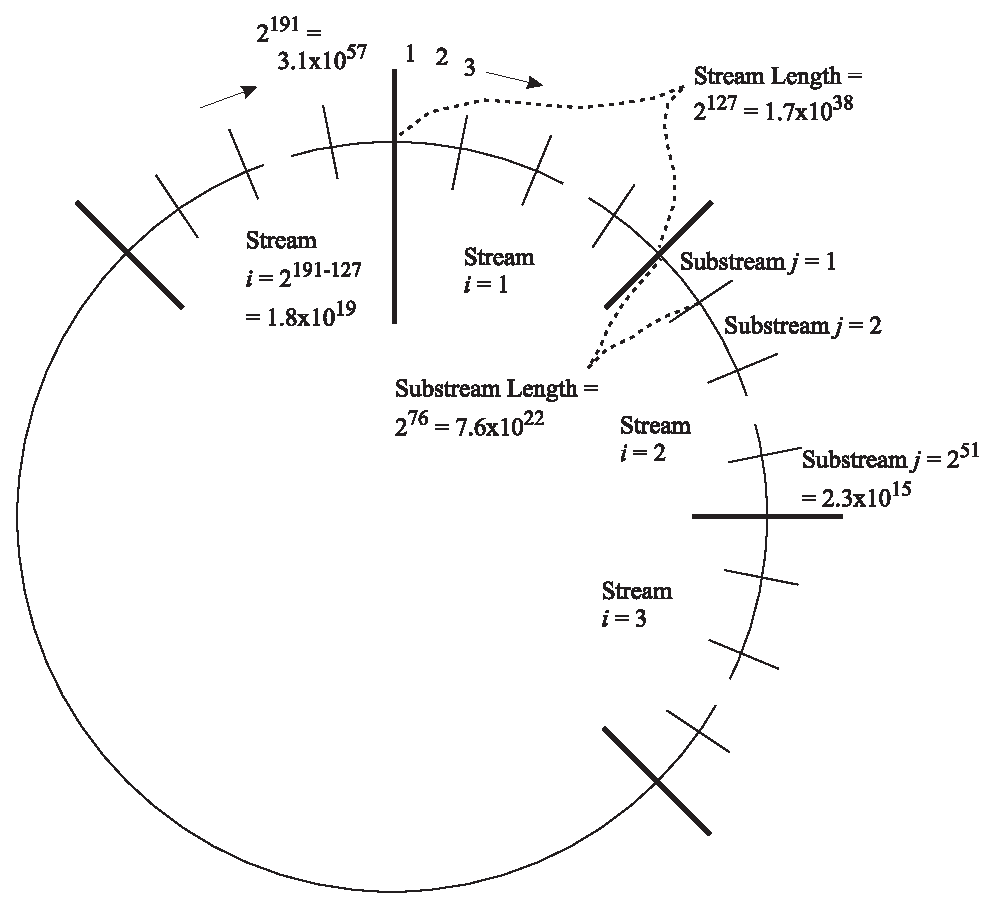
\psfig{file=fig2.eps,width=6.5in}}
\end{figure}
\fi  %%%%

Whenever a new stream is created (instantiated), say the $g^{th}$ stream, the software
automatically computes $I_g = T^Z(I_{g-1})$ and puts $C_g = B_g = I_g$.
When going from a substream to the next one, the software must compute
$N_g = T^W(B_g)$.
Of course, $W$ and $Z$ must be huge numbers, so a quick way to compute
$s_{n+\nu}$ from $s_n$ for large integers $\nu$, without generating
the intermediate values, must be available.
For a combined MRG, we can do this for each of its components separately,
as explained in \citeN{rLEC90a}:  % and \citeN{streams00l}:
one can write $s_{j,n+1} = A_j s_{j,n} \bmod m_j$ for some
$3\times 3$ matrix $A_j$, and then
\iflong %%%
$s_{j,n+\nu} = (A_j^\nu \bmod m_j) s_{j,n} \bmod m_j$, see Section \ref{avm}.
\else %%%
$s_{j,n+\nu} = (A_j^\nu \bmod m_j) s_{j,n} \bmod m_j$.
\fi %%%
The matrix $A_j^\nu \bmod m_j$ is computed via a standard divide-and-conquer
algorithm (\cite{rKNU98a}), and can be precomputed once
for $\nu = W$ and $\nu = Z$.
\iflong %%%
Most other random-number packages offer no
facility for jumping ahead directly from $s_{n}$ to $s_{n+\nu}$ or
to compute distant seeds efficiently.
\fi  %%%

%%%%%%%%%%%%
\subsection {Choice of $v$ and $w$}

We have selected $v=51$ and $w=76$, so $W = 2^{76}$ and $Z = 2^{127}$.
To select $v$ and $w$, a spectral test for
the vectors of {\em non-successive\/} output values
spaced $h=2^l$ steps apart was performed for different integer
values of $l$, and we chose $v$ and $w$ so that the behavior was
good for $l=v$, $l=w$, and $l=v+w$.
More specifically, let
$T_t(s,h)$ be the point set obtained if we replace $(u_n, \ldots,
u_{n+t-1})$ by the first $t$ components of the sequence
$(u_n,\ldots,
u_{n+s-1},u_h,\ldots,u_{n+h+s-1},u_{n+2h},\ldots,u_{n+2h+s-1},\ldots)$
in the definition of $T_t$.
If the streams are started $h$ apart,
the points of $T_t(s,h)$
%%  (except for the rescaling by $(m_1+1)/m_1$)
are those obtained by taking $s$ successive values from the first
stream, $s$ successive values from the second stream, and so on
until $t$ values have been taken.
\iflong  %%%%%%%%%
These points have a lattice structure and we have selected $l$ so
that it is good (the hyperplanes are close together) for
$h=2^l$ and (say) all $s \le 16$ and $t \le 32$. This was done for
$51 \le l \le 150$ and we found that the structure was
particularly good for $l=51,76$, and 127.
\else  %%%  (short)
We looked for values of $l$ such that for $h=2^l$,
the point set $T_t(s,h)$ was very uniformly distributed, according
to the spectral test, for all $s \le 16$ and $t \le 32$.
This was done for $51 \le l \le 150$ and we found that the
uniformity was particularly good for $l=51,76$, and 127.
\fi  %%%
%  We thus recommend $v=51$ and $w=76$, so $z=v+w=127$.

\iflong  %%%%%%%%%%%
\subsection {Precision and Speed of the RNG}  \label{precision}

Note that the generator gives no more than 32 bits of precision
even though it returns 53-bit floating-point numbers. If higher
precision is required, successive numbers produced by the
generator may be used to construct each output value. That is, if
the generator outputs the sequence $u_{1},u_{2},\ldots,$ one can
construct and use the sequence $v_{1},v_{2},\ldots,$ defined by
$$
  v_{i}=(vu_{2i}+u_{2i-1}) \bmod 1
$$
for some appropriate constant $v$, for instance $v=2^{-24}$.

Table~\ref{timing} gives the total elapsed time (in minutes) for
$10^9$ (one billion) calls to a given function from the package,
and the number of random numbers generated per second for certain
specific generators, on a Pentium III computer at 600MHz with
128MB of RAM, running Windows 98 and C++ codes compiled with
Microsoft visual C++ version 6.0. To get an idea of the
comparative speeds of the implementations, we also include the
timing of LCG {\tt lcgrand} of Law and Kelton (2000, pp.
430-431). Note that {\tt lcgrand} is implemented with integer
arithmetic. Furthermore, these one billion random numbers
represent almost half of the entire period of {\tt lcgrand}, which
would have been exhausted in about a half hour on our machine. The
absolute times of generating the random numbers are extremely
small and will be masked by other things going on in
most simulations. If we use Moore's law assuming that computing
speed doubles every 1.5 years, it will be approximately 219 years
into the future before average desktop computers will have the
capability to exhaust the cycle of {\tt RandU01} in a year of
continuous computing.

\begin {table}
\caption{Timing reports.}                         \label{timing}
\begin {center}
\begin {tabular}{lrr}
\hline
              &   Time to generate $10^9$  &  Random numbers       \\
  Function    &   random numbers (minutes) &  generated per second \\
\hline        &                            &                       \\
 RandU01      &      12.9                  &  1288659              \\
 RandU01 (inc. prec.) &      28.5          &   585480              \\
 RandInt      &      18.5                  &   901713              \\
 lcgrand      &      14.8                  &  1127395              \\
\hline
\end {tabular}
\end {center}
\end {table}

\fi  %%%%%%%%%%%%


\iflong  %%%%%%%%  For long version only.
%%%%%%%%%%%%%%%%%%%%%%%%%%%%%%%%%%%%%%%%%%%%%%%%%%%%%%%%%
\section {SUPPORT UTILITIES}
\label {utility}

Some random-number packages offer a limited
number of fixed streams, all based on the same generator, but
using fixed starting seeds set, say, 100,000 values apart. This
provides relatively low flexibility, as well as streams that are
far too short (close together) for modern computers (even PCs). A
simple procedure call should permit resetting a generator to a
previous seed or jumping ahead to a new seed for the next run.
Implementing such tools requires efficient jumping-ahead
facilities, which in turn requires efficient procedures to compute
the quantity $a \times s \bmod m$.

\subsection {Computing $a \times s \bmod m$}
\label {asm}

If the product $a\times s \le 2^{53}$, then it is always represented
exactly in floating point on 32-bit computers that support the
IEEE-754 floating-point arithmetic standard, with at least 53 bits
of precision for the mantissa. The generator can then be
implemented directly in floating-point arithmetic, which is
typically faster than an integer arithmetic implementation since
it is done in hardware on the CPU. On the other hand,
with this implementation, the state of the generator is
represented over 64 $k \times J$ bits, as opposed to 32 $k \times J$
bits when the $x_{j,n}$ are represented as 32-bit integers.

Now, consider a 32-bit computer on which all integers between $-2^{31}$
and $2^{31}$ (exclusive) are well represented. We want to compute $a \times s \bmod m$,
where $a$, $s$, and $m$ are positive integers smaller than $%
2^{32}$. Without loss of generality, we assume that $a<m$ and
$s<m$ (if not, replace $a$ and $s$ by $a \bmod m$ and $s \bmod m$,
respectively). Performing the computation is tricky, because the
product of $a\times s$ can exceed $2^{63}$, while double precision
in most 32-bit computers carries no more than 53 bits of accuracy.

An algorithm was developed to compute $a\times s \bmod m$ with
exact accuracy for the case where $a \times s > 2^{53}$
by making sure that no operations in the algorithm
produces a number greater than $2^{53}$.
A direct approach, based on decomposition, operates as follows.
Rewrite
\begin{eqnarray*}
a=a_{1}\times 2^{17}+a_{2},
\end{eqnarray*}
so $$ a\times s=a_{1}\times s \times 2^{17}+a_2\times s.$$
Therefore,
\begin{eqnarray*}
a\times s \bmod  m= ( (a_{1}\times s \bmod m) \times
2^{17}+a_2\times s) \bmod m
\end{eqnarray*}
where $a_1 < 2^{15}$, so $a_1 \times s < 2^{47} (=2^{15} \times
2^{32})$, $a_2 < 2^{17}$, and $a_2 \times s < 2^{49} (=2^{17}
\times 2^{32})$. Because $v=(a_{1}\times s \bmod m) < 2^{32}$, we
have $v \times 2^{17} < 2^{49}$ so that all the intermediate terms
in the above computations are less than $2^{53}.$ Therefore, all
seed values will have
%32-bit precision.
exact accuracy. Refer to function {\tt MultModM} in Appendix A for
an implementation of this algorithm.
Even though $a$, $s$, and $m$ are positive integers,
they are declared (and represented) as {\tt double}
internally in our C++ implementation.
% To access the values externally, {\tt unsigned long int}
% should be used.  ???

\subsection {Computing $A^{v} \bmod m$} \label {AmodM}
\label {avm}

The initial state of substreams can be computed easily if
jumping-ahead facilities are available for the individual MRG
components; that is, if an efficient algorithm is available for
computing the state of the MRG $v$ steps ahead of the current one,
for large values of $v$.
\citeN{rLEC90a} % L'Ecuyer (1990)
explains one way of doing
that, based on the fact that the MRG can be viewed as a LCG
in matrix form, whose state is a
$k$-dimensional vector and whose multiplier is a $k\times k$
matrix $A$. To jump ahead by $v$ values, just multiply the current
state by $A^{v} \bmod m$. The matrix $A^{v} \bmod m$ can be
pre-computed in time O(log $v$), using the divide-and-conquer
algorithm (\cite{iBRA88a,rKNU98a,rLEC96b}).
%  Brassard and Bratley 1988; Knuth 1998; L'Ecuyer 1996).

That is, for the MRG, $s_{n+v}$ can be
computed directly from $s_{n}$ using
\begin{eqnarray}
s_{n+v}=(A^{v}s_{n}) \bmod m
=(A^{v} \bmod m)s_{n} \bmod m
\end{eqnarray}
where
\begin{eqnarray}
A= \left(
\begin{array}{cccc}
0 & 1 & \cdot & 0 \\
\cdot & \cdot & \cdot & \cdot \\
0 & 0 & \cdot & 1 \\
a_{k} & a_{k-1} & \cdot & a_{1}
\end{array}
\right ).
\end{eqnarray}
When $A$ has this special structure, the first $k-1$ components of
$s_{n}$ are obtained by shifting the last $k-1$ components of
$s_{n-1}$, and the last component of $s_{n}$ is a linear
combination of the components of $s_{n-1}$ according to the MRG
recursion (\cite{rLEC90a}).

Thus, in our implementation the matrix $A_1$ for $s_{1,n}$ to jump ahead one step is
$$
A_1 = \left (
\begin{array}{ccc}
0 & 1 & 0 \\
0 & 0 & 1 \\
-810728 & 1403580 & 0
\end{array}
\right ) $$ and the matrix $A_2$ for $s_{2,n}$ to jump ahead one
step is $$ A_2 = \left (
\begin{array}{ccc}
0 & 1 & 0 \\
0 & 0 & 1 \\
-1370589 & 0 & 527612
\end{array}
\right ).
$$



The divide-and-conquer algorithm computes the jump-ahead matrix
$A^{v}$ using the following recursion:
\[ A^v \bmod m =
\left\{
\begin{array}{ll}
A                              & \mbox{if $v=1$;}\\
A \times A^{v-1} \bmod m       & \mbox{if $v>1$, $v$ odd;} \\
A^{v/2} \times A^{v/2} \bmod m & \mbox{if $v > 1$, $v$ even.}
\end{array}
\right. \]

See the procedure {\tt MatPowModM} in Appendix A for an implementation
of this algorithm for a $3\times 3$ matrix.

%%%%%%%%%%%
\subsection {Jumping Backward}                 \label{backward}

Fermat's first theorem tells us that $A_j^{\rho_j} \bmod m_j=I$,
where $\rho_j$ is the period length of the $j^{th}$ MRG component,
because each component has a primitive characteristic polynomial.
Therefore, $B_j = A_j^{\rho_j -1} \bmod m_j$ is the multiplicative
inverse of $A_j \bmod m_j$.
This means that $B_j$ is the jump-back-one-step matrix:
Given a vector $s_{j,n}$, one can jump back $v$ steps to
$s_{j,n-v}$ by multiplying $s_{j,n}$ by $B_j^v$.
The matrix $B_j$ generates the same stream but in reverse order.
As we can see from the new recursion below, the
values of the parameters $b_{ij}$ are much larger than the
original ones, where the $b_{ij}$ are the parameters of the new CMRG.
Furthermore, we no longer have $b_{ij} (m_j-1) < 2^{53}$ for all
$b_{ij}$, so that the implementation would be slower than that of the
original recursion.

The matrix $B_1$ for $s_{1,n}$ to jump back one step is
$$ B_1 =
\left (
\begin{array}{ccc}
184888585 & 0 & 1945170933 \\
1 & 0 & 0 \\
0 & 1 & 0
\end{array}
\right ) $$ and for $s_{2,n}$ to jump back one step we have $$ B_2
= \left (
\begin{array}{ccc}
0 & 360363334 & 4225571728 \\
1 & 0 & 0 \\
0 & 1 & 0
\end{array}
\right ).
$$
The reverse stream follows the recursion
\begin {eqnarray*}
 x_{1,n} &=& (184888585\times x_{1,n+1}+1945170933\times x_{1,n+3})
              \bmod 4294967087, \\
 x_{2,n} &=& (360366334\times x_{2,n+2}+4225571728\times x_{2,n+3})
              \bmod 4294944443 \\
   &=& (360366334\times x_{2,n+2}-69372715\times x_{2,n+3})
         \bmod 4294944443.
\end {eqnarray*}

\fi  %%%%%%%%%    End of ``support utilities''.

\iflong  %%%%%%%%
%%%%%%%%%%%%%%%%%%%%%%%%%%%%%%%%%%%%%%%%%%%%%%%%%%%%%%%%%%%%%%%%%%%%
\section {A PORTABLE AND EFFICIENT PACKAGE FOR RANDOM-NUMBER GENERATION}
\label {RNG}

We now provide a set of portable utilities for random-number
generation. The initial values of ($x_{1,0},x_{1,1},x_{1,2}$) can
be any non-negative integer values less than $m_{1}$ and not all
zero, and the initial values of ($x_{2,0},x_{2,1},x_{2,2}$) can be
any non-negative integer values less than $m_{2}$ and not all
zero.

The initial seed of the main generator $s_0$ is the starting point
of the first stream $I_1$. In the proposed package, the initial
seed $s_{0}=I_{1}$ is set to the
 default value $(12345, 12345, 12345, 12345,$ $12345, 12345)$,
but this value can be changed by the user (via
 {\tt SetPackageSeed}). Each time a new
 {\tt RngStream} object is created, its starting point (initial seed)
$I_g$ is set $Z=2^{127}$ steps ahead of the starting point of
the last created object.
A vector named {\tt nextSeed} is used to keep
the seed values of the next created  {\tt RngStream} object (stream).
For example, the declaration ``{\tt RngStream g;}''
creates a stream with $I_g$ equal to {\tt
nextSeed} and advances {\tt nextSeed} by $Z$ steps. Because the
initial seed for each {\tt RngStream} object is computed
dynamically, no pre-computed list of seeds is needed.

For each {\tt RngStream}, one can generate one value and go ahead
one step, or go ahead to the beginning of the next substream
within this stream, or go back to the beginning of the current
substream, or to the beginning of the stream, or jump ahead or
back by an arbitrary number of steps.
As discussed in Section \ref{backbone}, the spacing between adjacent
substreams is $W=2^{76}$.
To get a feel for the extent of these spacings of streams and
substreams, it would take over 1.8 billion years for {\tt RandU01}
to exhaust one of the substreams using the hardware producing the
timings of Table~\ref{timing}.  Once again assuming that Moore's
law will continue to hold, {\tt RandU01} will require two months
on an average desktop computer 50 years from now to exhaust one of
the substreams (but over 385 millennia to exhaust one of the
streams).

Several pre-computed jump matrices are provided in the  {\tt RngStream}
class. With these jump matrices, we are able to compute the
initial seed for each stream dynamically and reset the stream to
various states. Thus, each instance of {\tt RngStream} can assume
different disjoint streams of which there are $2^{64} \approx 1.8
\times 10^{19}$ (so are virtually unlimited). Moreover, one can
use {\tt AdvanceState} to jump ahead or backward.

The methods {\tt Reset*} reset a given stream either to its
initial state ($C_g \leftarrow I_g$ and $B_g \leftarrow I_g$), or
to the beginning of its current substream ($C_g \leftarrow B_g$),
or to the beginning of its next substream ($C_g \leftarrow N_g$
and $B_g \leftarrow N_g$). The method {\tt GetState} returns
the state of a stream. One can change the seed of a given stream,
without modifying that of other streams, by invoking {\tt SetSeed}
or {\tt AdvanceState}. However, after calling {\tt SetSeed} for a
given stream, the initial states of the different streams are no
longer spaced $Z$ values apart. Therefore, this method should be
used {\em only in exceptional cases}.
The methods {\tt Reset*} suffices for almost all applications.

The methods {\tt RandU01} and {\tt RandInt}
generate the uniform (pseudo)random numbers. Each stream can
produce (if desired) {\em antithetic\/} random numbers with respect
to the uniforms normally produced, i.e., return $1-U$ instead of
$U$, by calling {\tt SetAntithetic}, or produce
53-bit precision random numbers by calling {\tt IncreasePrecis}.

Here are examples of situations where the tools offered in this
package are useful:

\begin{itemize}
\item
Compare two or more similar systems, via simulation with common
random numbers, with $n$ simulation runs for each system. To
guarantee that the same random numbers are used across the systems
with good synchronization, assign different streams to different
places where random numbers are needed in the model (e.g., to
compare queuing systems, use one stream for interarrival times,
one stream for the service times at each queue, one stream for a
routing decision, etc.). To make sure that each stream starts from
the same state across the different systems, assign run $j$ to the
$j^{th}$ substream, within each stream. The experiment then
proceeds as follows. For the first system, simulate run 1 by
starting all the streams from their initial seed, $I_g$. Before
each new run, advance all the streams to the initial state of
their next substream, $N_g$. After the $n^{th}$ run, reset all the
streams to their initial state, $I_g$. Repeat for each system to
compare; see Example 2 in Section \ref{example}. Note that in this
application, the substreams correspond to replications within each
stream.

\item
Run simulations on several processors, in parallel, and each
processor is to have its own (virtual) generator. In this case,
simply use one stream for each processor. There must be a central
authority, or {\em monitor}, to manage the allocation of the
streams, but once a stream is allocated, the processors can go
their own way, independently of each other. In this setup, the
processors in fact use the same generator, but with different {\em
seeds}. This makes the implementation much easier than if a
different generator must be implemented on each processor.

\end{itemize}

\else  %%%

%%%%%%%%%%%%%%%%%%%%%%%%%%%%%%%%%%%%%%%%%%%%%%%%%%%%
\section {A C++ INTERFACE TO THE PACKAGE RNGSTREAMS}
\label {sec:interface}

\fi  %%%%%

\iflong %%%
We now describe the
members of the C++  class {\tt RngStream}.
This is the file {\tt RngStream.h}, with comments.
\else  %%%
We now describe the main public members of the class {\tt
RngStream} in C++. Other methods and further details are available
in the Online Companion to this paper on the {\it Operations %wdk
Research\/} website. %wdk
\fi  %%%

%%%%%%%%%%%%%%%%%%%%%%%%%%%%%%%%%%%%%%%%%%%%%%%%%
%%  File RngStream.tex starts here

\code
\hide
#ifndef RNGSTREAM_H
#define RNGSTREAM_H
\endhide
#include <string>

class RngStream
{
public:

RngStream (const char *name = "");
\endcode
 \tab This constructor  %% of the {\tt RngStream} class
 creates a new stream with (optional) descriptor {\tt name}.
 It initializes its seed $I_g$, and sets $B_g$ and $C_g$ to $I_g$.
\iflong %%
 It also sets its {\tt anti} and {\tt incPrec} switches to {\tt false}.
\fi %%
  The seed $I_g$ is equal to the initial seed of the package
% given by {\tt SetPackageSeed}
  if this is the first stream created;
   otherwise it is $Z$ steps ahead of the seed of the most recently
   created stream.
% If the method {\tt SetPackageSeed} has
% not been called, the first created stream will have the default seed
% (12345, 12345, 12345, 12345, 12345, 12345).
 \endtab
\code

static bool SetPackageSeed (const unsigned long seed[6]);
\endcode
 \tab Sets the initial seed $s_0$ of the package to the six integers
   in the vector {\tt seed}.
   The first 3 integers in the seed must all be
   less than $m_1 = 4294967087$, and not all 0;
   and the last 3 integers
   must all be less than $m_2 = 4294944443$, and not all 0.
%   This will be the seed (initial state) of the first stream.
   If this method is not called, the default initial seed
   is (12345, 12345, 12345, 12345, 12345, 12345).
   Returns {\tt false} for invalid seeds, and  {\tt true} otherwise.
 \endtab
\code

void ResetStartStream ();
\endcode
 \tab Reinitializes the stream to its initial state:
   $C_g$ and $B_g$ are set to $I_g$.
 \endtab
\code

void ResetStartSubstream ();
\endcode
 \tab Reinitializes the stream to the beginning of its current
   substream: $C_g$ is set to $B_g$.
 \endtab
\code

void ResetNextSubstream ();
\endcode
 \tab Reinitializes the stream to the beginning of its next
   substream: $N_g$ is computed, and
   $C_g$ and $B_g$ are set to $N_g$.
 \endtab
\code

void SetAntithetic (bool a);
\endcode
 \tab  If {\tt a = true}, the stream will start generating
 antithetic variates, i.e., $1-U$ instead of $U$, until this method is
 called again with {\tt a = false}.
% By default, the streams are created with {\tt anti = false}.
 \endtab
\code

void IncreasedPrecis (bool incp);
\endcode
 \tab After calling this method with {\tt incp = true}, each call to
  the generator (direct or indirect) for this stream
  will return a uniform random number with more bits of resolution
  (53 bits if machine follows IEEE 754 standard) instead of 32 bits,
  and will advance the state of the stream by 2 steps instead of 1.
  More precisely, if {\tt s} is a stream of the class {\tt RngStream},
  in the non-antithetic case, the instruction
  ``{\tt u = s.RandU01()}'' will be equivalent to
  ``{\tt u = (s.RandU01() + s.RandU01() * fact) \%\ 1.0}''
  where the constant {\tt fact} is equal to $2^{-24}$.
  This also applies when calling {\tt RandU01} indirectly
  (e.g., via {\tt RandInt}, etc.).
  By default, or if this method is called again with {\tt incp = false},
  each call to {\tt RandU01} for this stream advances the state by 1 step
  and returns a number with 32 bits of resolution.
 \endtab
\iflong %%%%%%%
\code

bool SetSeed (const unsigned long seed[6]);
\endcode
 \tab  Sets the initial seed $I_g$ of the stream to
 the vector {\tt seed}. The vector {\tt seed}
 should contain valid seed values as described in {\tt
 SetPackageSeed}. The state of the stream is then reset
 to this initial seed. The states and seeds of the other
 streams are not modified. As a result, after calling this
 method, the initial seeds of the streams are no longer spaced
 $Z$ values apart. We discourage the use of this method; proper
 use of the {\tt Reset*} methods is preferable.
   Returns {\tt false} for invalid seeds, and  {\tt true} otherwise.
 \endtab
\code

void AdvanceState (long e, long c);
\endcode
 \tab  Advances the state by
  $n$ steps (see below for the meaning of $n$), without modifying
  the states of other streams or the values of $B_g$ and $I_g$ in
  the current object. If ${\tt e} > 0$, then $n = 2^{\tt e} + {\tt c}$;
  if ${\tt e} < 0$, then $n=-2^{\tt -e}+{\tt c}$; and if ${\tt e=0}$,
  then $n={\tt c}$. Note: {\tt c} is allowed to take negative values.
  We discourage the use of this method.
 \endtab
\code

void GetState (unsigned long seed[6]) const;
\endcode
 \tab  Returns in {\tt seed[0..5]} the current state
 $C_g$ of this stream. This is convenient if we want to
 save the state for subsequent use.
 \endtab
\fi  %%%%%%%
\code

void WriteState () const;
\endcode
 \tab  Writes (to standard output) the current
 state $C_g$ of this stream.
 \endtab
\iflong %%%%%%
\code

void WriteStateFull () const;
\endcode
 \tab  Writes (to standard output) the value
 of all the internal variables of this stream:
  {\tt name, anti, incPrec, Ig, Bg, Cg}.
 \endtab
\fi  %%%%%%
\code

double RandU01 ();
\endcode
 \tab Normally, returns a (pseudo)random number from the uniform distribution
   over the interval $(0,1)$, after advancing the state by one step.
   The returned number has 32 bits of precision in the sense that it is
   always a multiple of $1/(2^{32}-208)$.
   However, if {\tt IncreasedPrecis(true)} has been called
   for this stream, the state is advanced by two steps and the returned
   number has 53 bits of precision.
 \endtab
\code

int RandInt (int i, int j);
\endcode
 \tab  Returns a (pseudo)random number from the discrete uniform
   distribution over the integers $\{i,i+1,\dots,j\}$.
   Makes one call to {\tt RandU01}.
 \endtab
\iflong %%%%%   Why put this here instead of hide it in the code?
\code


private:

double Cg[6], Bg[6], Ig[6];
\endcode
 \tab Vectors to store the current seed, the beginning of the current
   block (substream) and the beginning of the current stream.
 \endtab
\code

bool anti, incPrec;
\endcode
 \tab Variables to indicate whether to generate antithetic or increased
   precision random numbers.
 \endtab
\code

std::string name;
\endcode
 \tab String to store the optional name of the current {\tt RngStream}
  object.
 \endtab
\code

static double nextSeed[6];
\endcode
 \tab Static vector to store the beginning state of the next
  {\tt RngStream} to be created (instantiated).
 \endtab
\code

double U01 ();
\endcode
 \tab The backbone uniform random number generator.
 \endtab
\code

double U01d ();
\endcode
 \tab The backbone uniform random number generator with increased precision.
 \endtab
\fi %%%
\code

};
\hide
#endif
\endhide
\endcode

%% File RngStream.tex ends here

%\iffalse %%%%%%%%%%%%%
\iflong %%%

%%%%%%%%%%%%%%%%%%%%%%%%%%%%%%%%%%%%%%%%%%%%%%%%%%%%%%%%%%%
\section {EXAMPLES}
\label{example}

Example1.c in Figure~\ref{example1} shows how we generate a list
of ten seed vectors. We
set the package seed to \{327612383, 317095578, 14704821,
 884064067, 1017894425, 16401881\} by calling {\tt SetPackageSeed}
before instantiating any  {\tt RngStream} object. Note that if
 {\tt SetPackageSeed} is not executed, \{12345, 12345, 12345, 12345,
12345, 12345\} will be used as the default package seed. The
declaration ``{\tt RngStream RngObj}'' is inside the {\tt for} loop
on $i$. Therefore, the instance of the object dies before the next
iteration, i.e., the object {\tt RngObj} is not available outside
the {\tt for} loop on $i$. Each declaration will create the {\tt
RngObj} instance with $I_g=B_g=C_g={\tt nextSeed}$ and advance
{\tt nextSeed} by $2^{127}$ steps. Thus, the output seeds will be
$2^{127}$ apart.

\begin{figure}[hbt]
\caption{example1.C.} \label{example1}
\begin{verbatim}
#include "RngStream.h"

int main ()
{
   unsigned long seed[6] = { 327612383, 317095578, 14704821,
                             884064067, 1017894425, 16401881 };
   RngStream::SetPackageSeed (seed);

   for (int i = 1; i <= 10; ++i) {
      RngStream RngObj;
      RngObj.WriteState();
   };
}
\end{verbatim}
\end{figure}

\sesquispace
\hspace{18pt}
Example2.c in Figure~\ref{example2} shows how to apply some of the
utilities supplied in the package. The declarations ``{\tt
RngStream RngObj1}'' and ``{\tt RngStream RngObj2}'' will create the
RNG objects with
$$I_g=B_g=C_g=\{12345, 12345, 12345, 12345,
  12345, 12345\}$$
and
$$I_g=B_g=C_g=\{3692455944, 1366884236,
 2968912127, 335948734, 4161675175, 475798818\},$$
respectively, i.e., $2^{127}$ steps apart.
The first RNG object {\tt RngObj1} may be dedicated to generate
interarrival times while the second RNG object {\tt RngObj2} may
be dedicated to generate service times, for some queueing system
to be simulated.
We generate five interarrival times and five service times,
then move each RNG to its next substream.
% i.e., the $B_g$ for each RNG object will be $2^{76}$ apart
% for each iteration in the {\tt for} loop on $j$.
This is repeated ten times, thus yielding ten vectors,
each containing five interarrival times and five service times.
Moreover, these ten vectors will be exactly the same at
iterations $k=0$ and $k=1$ of the outer {\tt for} loop,
because the statements ``{\tt RngObj1.ResetStartStream}'' and
``{\tt RngObj2.ResetStartStream}'' will reset the current seeds
$C_g$ of both RNG objects to the initial seed $I_g$.

\begin{figure}[htb]
\caption{example2.C.} \label{example2}
\begin{verbatim}
#include <math.h>
#include "RngStream.h"

int main ()
{
   RngStream RngObj1;
   RngStream RngObj2;
   double interArrival;
   double serviceTime;

   for (int k = 0; k <= 1; ++k) {
      for (int j = 1; j <= 10; ++j) {
         for (int i = 1; i <= 5; ++i) {
             interArrival = -log (1.0 - RngObj1.RandU01());
             serviceTime  = -0.9 * log (1.0 - RngObj2.RandU01());
         };
         RngObj1.ResetNextSubstream ();
         RngObj2.ResetNextSubstream ();
      };
      RngObj1.ResetStartStream ();
      RngObj2.ResetStartStream ();
   };
}
\end{verbatim}
\end{figure}

%%%%%%%%%%%%%%%%%%%%%%%%%%%%%%%%%%%%%%%%%%%%%%%%%%%%%%%%
\section{SUMMARY}
\label{summary}

We have discussed the backbone CMRG random-number generator,
several utilities to enhance its practical use, and implementation
issues. We briefly mentioned how the spacing between each stream
was chosen, based on a lattice-structure analysis of its
successive output values. We implemented a RNG package in the C++
language. Our implementation eliminates the need to use a fixed
number of pre-computed seeds, which would provide little
flexibility. The proposed RNG package
provides jumping facilities, has good speed, a long period,
and excellent theoretical/statistical properties.

\fi  %%%%%%%%%%

%%%%%%%%%%%%%%%%%%%%%%%%%%%%%%%%%%%%%%%%%%%%%%%%%%%%%%%%%%%
\section*{ACKNOWLEDGMENTS}

This work has been supported by NSERC-Canada grant number
ODGP0110050 to the first author.
\iflong %%
We thank C. Dennis Pegden for suggesting the type of
depiction in Figure~\ref{streams}.
\fi %%

%%%%%%%%%%%%%%%%%%%%%%%%%%%%%%%%%%
\section*{REFERENCES}

%\bibliography {random,simul,math,ift}
\bibliographystyle {opres}

%%%  The following is a patch because you don't have my .bib databases.

\iflong  %%%%%%
\begin{refer}

\bibitem[Brassard and Bratley][1988]{iBRA88a}
Brassard, G and P.~Bratley. 1988.
\newblock {\em Algorithmics, Theory and Practice}.
\newblock Prentice-Hall.

\bibitem[Knuth][1998]{rKNU98a}
Knuth, D.~E. 1998.
\newblock {\em The Art of Computer Programming, Volume 2: Seminumerical
  Algorithms}.
\newblock Third ed. Reading, Mass.: Addison-Wesley.

\bibitem[Law and Kelton][2000]{sLAW00a}
Law, A.~M and W.~D. Kelton. 2000.
\newblock {\em Simulation Modeling and Analysis}.
\newblock Third ed. New York: McGraw-Hill.

\bibitem[L'Ecuyer][1990]{rLEC90a}
L'Ecuyer, P. 1990.
\newblock Random numbers for simulation.
\newblock {\em Communications of the ACM},  {\bf 33}(10), 85--97.

\bibitem[L'Ecuyer][1996]{rLEC96b}
L'Ecuyer, P. 1996.
\newblock Combined multiple recursive random number generators.
\newblock {\em Operations Research},  {\bf 44}(5), 816--822.

\bibitem[L'Ecuyer][1999a]{rLEC99b}
L'Ecuyer, P. 1999a.
\newblock Good parameters and implementations for combined multiple recursive
  random number generators.
\newblock {\em Operations Research},  {\bf 47}(1), 159--164.

\bibitem[L'Ecuyer][1999b]{rLEC99a}
L'Ecuyer, P. 1999b.
\newblock Tables of maximally equidistributed combined {LFSR} generators.
\newblock {\em Mathematics of Computation},  {\bf 68}(225), 261--269.

\bibitem[L'Ecuyer and Andres][1997]{rLEC97d}
L'Ecuyer, P and T.~H. Andres. 1997.
\newblock A random number generator based on the combination of four {LCG}s.
\newblock {\em Mathematics and Computers in Simulation},  {\bf 44}, 99--107.

\bibitem[L'Ecuyer and C{\^o}t{\'e}][1991]{rLEC91a}
L'Ecuyer, P. and S.~C{\^o}t{\'e}. 1991.
\newblock Implementing a random number package with splitting facilities.
\newblock {\em ACM Transactions on Mathematical Software},  {\bf 17}(1),
  98--111.

\bibitem[L'Ecuyer and Simard][2001]{rLEC01a}
L'Ecuyer, P. and R.~Simard. 2001.
\newblock On the performance of birthday spacings tests for certain families of
  random number generators.
\newblock {\em Mathematics and Computers in Simulation},  {\bf 55}(1--3),
  131--137.

\bibitem[L'Ecuyer et~al.][2001]{rLEC01s}
L'Ecuyer, P., R.~Simard, E.~J. Chen, and W.~D. Kelton. 2001.
\newblock An object-oriented random-number package with many long streams and
  substreams.
\newblock Submitted.

\bibitem[Marsaglia][1985]{rMAR85a}
Marsaglia, G. 1985.
\newblock A current view of random number generators.
\newblock In {\em Computer Science and Statistics, Sixteenth Symposium on the
  Interface}, 3--10, North-Holland, Amsterdam. Elsevier Science Publishers.

\bibitem[Mascagni and Srinivasan][2000]{rMAS00a}
Mascagni, M and A.~Srinivasan. 2000.
\newblock Algorithm 806: {SPRNG}: A scalable library for pseudorandom number
  generation.
\newblock {\em {ACM} Transactions on Mathematical Software},  {\bf 26},
  436--461.

\bibitem[Matsumoto and Nishimura][1998]{rMAT98a}
Matsumoto, M. and T.~Nishimura. 1998.
\newblock Mersenne twister: A 623-dimensionally equidistributed uniform
  pseudo-random number generator.
\newblock {\em ACM Transactions on Modeling and Computer Simulation},  {\bf
  8}(1), 3--30.

\end{refer}

\else  %%%%%

\begin{refer}

\bibitem[Knuth][1998]{rKNU98a}
Knuth, D.~E. 1998.
\newblock {\em The Art of Computer Programming, Volume 2: Seminumerical
  Algorithms}.
\newblock Third ed. Reading, Mass.: Addison-Wesley.

\bibitem[Law and Kelton][2000]{sLAW00a}
Law, A.~M and W.~D. Kelton. 2000.
\newblock {\em Simulation Modeling and Analysis}.
\newblock Third ed. New York: McGraw-Hill.

\bibitem[L'Ecuyer][1990]{rLEC90a}
L'Ecuyer, P. 1990.
\newblock Random numbers for simulation.
\newblock {\em Communications of the ACM},  {\bf 33}(10), 85--97.

\bibitem[L'Ecuyer][1999a]{rLEC99b}
L'Ecuyer, P. 1999a.
\newblock Good parameters and implementations for combined multiple recursive
  random number generators.
\newblock {\em Operations Research},  {\bf 47}(1), 159--164.

\bibitem[L'Ecuyer][1999b]{rLEC99a}
L'Ecuyer, P. 1999b.
\newblock Tables of maximally equidistributed combined {LFSR} generators.
\newblock {\em Mathematics of Computation},  {\bf 68}(225), 261--269.

\bibitem[L'Ecuyer and Andres][1997]{rLEC97d}
L'Ecuyer, P and T.~H. Andres. 1997.
\newblock A random number generator based on the combination of four {LCG}s.
\newblock {\em Mathematics and Computers in Simulation},  {\bf 44}, 99--107.

\bibitem[L'Ecuyer and C{\^o}t{\'e}][1991]{rLEC91a}
L'Ecuyer, P. and S.~C{\^o}t{\'e}. 1991.
\newblock Implementing a random number package with splitting facilities.
\newblock {\em ACM Transactions on Mathematical Software},  {\bf 17}(1),
  98--111.

\bibitem[L'Ecuyer and Simard][2001]{rLEC01a}
L'Ecuyer, P. and R.~Simard. 2001.
\newblock On the performance of birthday spacings tests for certain families of
  random number generators.
\newblock {\em Mathematics and Computers in Simulation},  {\bf 55}(1--3),
  131--137.

\bibitem[Mascagni and Srinivasan][2000]{rMAS00a}
Mascagni, M. and A.~Srinivasan. 2000.
\newblock Algorithm 806: {SPRNG}: A scalable library for pseudorandom number
  generation.
\newblock {\em {ACM} Transactions on Mathematical Software},  {\bf 26},
  436--461.

\bibitem[Matsumoto and Nishimura][1998]{rMAT98a}
Matsumoto, M. and T.~Nishimura. 1998.
\newblock Mersenne twister: A 623-dimensionally equidistributed uniform
  pseudo-random number generator.
\newblock {\em ACM Transactions on Modeling and Computer Simulation},  {\bf
  8}(1), 3--30.

\end{refer}

\fi  %%%%

%%%%%  Short version is over.
\iflong %%%%%%
\newpage

%%%%%%%%%%%%%%%%%%%%%%%%%%%%%%%%%%%%%%%%%%%%%%%%%%%%%%%%%%%%
\appendix
\section*{APPENDIX A. \ A C++ IMPLEMENTATION}
\singlespace

\begin{verbatim}
/***********************************************************************\
 *
 * File:           RngStream.cpp for multiple streams of Random Numbers
 * Language:       C++ (ISO 1998)
 * Copyright:      Pierre L'Ecuyer, University of Montreal
 * Notice:         This code can be used freely for personal, academic,
 *                 or non-commercial purposes. For commercial purposes, 
 *                 please contact P. L'Ecuyer at: lecuyer@iro.umontreal.ca
 * Date:           14 August 2001
 *
\***********************************************************************/


#include <cstdlib>
#include <iostream>
#include "RngStream.h"
using namespace std;

namespace
{
const double m1   =       4294967087.0;
const double m2   =       4294944443.0;
const double norm =       1.0 / (m1 + 1.0);
const double a12  =       1403580.0;
const double a13n =       810728.0;
const double a21  =       527612.0;
const double a23n =       1370589.0;
const double two17 =      131072.0;
const double two53 =      9007199254740992.0;
const double fact =       5.9604644775390625e-8;     /* 1 / 2^24  */

// The following are the transition matrices of the two MRG components
// (in matrix form), raised to the powers -1, 1, 2^76, and 2^127, resp.

const double InvA1[3][3] = {          // Inverse of A1p0
       { 184888585.0,   0.0,  1945170933.0 },
       {         1.0,   0.0,           0.0 },
       {         0.0,   1.0,           0.0 }
       };

const double InvA2[3][3] = {          // Inverse of A2p0
       {      0.0,  360363334.0,  4225571728.0 },
       {      1.0,          0.0,           0.0 },
       {      0.0,          1.0,           0.0 }
       };

const double A1p0[3][3] = {
       {       0.0,        1.0,       0.0 },
       {       0.0,        0.0,       1.0 },
       { -810728.0,  1403580.0,       0.0 }
       };

const double A2p0[3][3] = {
       {        0.0,        1.0,       0.0 },
       {        0.0,        0.0,       1.0 },
       { -1370589.0,        0.0,  527612.0 }
       };

const double A1p76[3][3] = {
       {      82758667.0, 1871391091.0, 4127413238.0 },
       {    3672831523.0,   69195019.0, 1871391091.0 },
       {    3672091415.0, 3528743235.0,   69195019.0 }
       };

const double A2p76[3][3] = {
       {    1511326704.0, 3759209742.0, 1610795712.0 },
       {    4292754251.0, 1511326704.0, 3889917532.0 },
       {    3859662829.0, 4292754251.0, 3708466080.0 }
       };

const double A1p127[3][3] = {
       {    2427906178.0, 3580155704.0,  949770784.0 },
       {     226153695.0, 1230515664.0, 3580155704.0 },
       {    1988835001.0,  986791581.0, 1230515664.0 }
       };

const double A2p127[3][3] = {
       {    1464411153.0,  277697599.0, 1610723613.0 },
       {      32183930.0, 1464411153.0, 1022607788.0 },
       {    2824425944.0,   32183930.0, 2093834863.0 }
       };



//-------------------------------------------------------------------------
// Return (a*s + c) MOD m; a, s, c and m must be < 2^35
//
double MultModM (double a, double s, double c, double m)
{
    double v;
    long a1;

    v = a * s + c;

    if (v >= two53 || v <= -two53) {
        a1 = static_cast<long> (a / two17);    a -= a1 * two17;
        v  = a1 * s;
        a1 = static_cast<long> (v / m);     v -= a1 * m;
        v = v * two17 + a * s + c;
    }

    a1 = static_cast<long> (v / m);
    /* in case v < 0)*/
    if ((v -= a1 * m) < 0.0) return v += m;   else return v;
}


//-------------------------------------------------------------------------
// Compute the vector v = A*s MOD m. Assume that -m < s[i] < m.
// Works also when v = s.
//
void MatVecModM (const double A[3][3], const double s[3], double v[3],
                 double m)
{
    int i;
    double x[3];               // Necessary if v = s

    for (i = 0; i < 3; ++i) {
        x[i] = MultModM (A[i][0], s[0], 0.0, m);
        x[i] = MultModM (A[i][1], s[1], x[i], m);
        x[i] = MultModM (A[i][2], s[2], x[i], m);
    }
    for (i = 0; i < 3; ++i)
        v[i] = x[i];
}


//-------------------------------------------------------------------------
// Compute the matrix C = A*B MOD m. Assume that -m < s[i] < m.
// Note: works also if A = C or B = C or A = B = C.
//
void MatMatModM (const double A[3][3], const double B[3][3],
                 double C[3][3], double m)
{
    int i, j;
    double V[3], W[3][3];

    for (i = 0; i < 3; ++i) {
        for (j = 0; j < 3; ++j)
            V[j] = B[j][i];
        MatVecModM (A, V, V, m);
        for (j = 0; j < 3; ++j)
            W[j][i] = V[j];
    }
    for (i = 0; i < 3; ++i)
        for (j = 0; j < 3; ++j)
            C[i][j] = W[i][j];
}


//-------------------------------------------------------------------------
// Compute the matrix B = (A^(2^e) Mod m);  works also if A = B. 
//
void MatTwoPowModM (const double A[3][3], double B[3][3], double m, long e)
{
   int i, j;

   /* initialize: B = A */
   if (A != B) {
      for (i = 0; i < 3; ++i)
         for (j = 0; j < 3; ++j)
            B[i][j] = A[i][j];
   }
   /* Compute B = A^(2^e) mod m */
   for (i = 0; i < e; i++)
      MatMatModM (B, B, B, m);
}


//-------------------------------------------------------------------------
// Compute the matrix B = (A^n Mod m);  works even if A = B.
//
void MatPowModM (const double A[3][3], double B[3][3], double m, long n)
{
    int i, j;
    double W[3][3];

    /* initialize: W = A; B = I */
    for (i = 0; i < 3; ++i)
        for (j = 0; j < 3; ++j) {
            W[i][j] = A[i][j];
            B[i][j] = 0.0;
        }
    for (j = 0; j < 3; ++j)
        B[j][j] = 1.0;

    /* Compute B = A^n mod m using the binary decomposition of n */
    while (n > 0) {
        if (n % 2) MatMatModM (W, B, B, m);
        MatMatModM (W, W, W, m);
        n /= 2;
    }
}


//-------------------------------------------------------------------------
// Check that the seeds are legitimate values. Returns 0 if legal seeds,
// -1 otherwise.
//
int CheckSeed (const unsigned long seed[6])
{
    int i;

    for (i = 0; i < 3; ++i) {
        if (seed[i] >= m1) {
            cerr << "****************************************\n"
                 << "ERROR: Seed[" << i << "] >= 4294967087, Seed is not set."
                 << "\n****************************************\n\n";
            return (-1);
        }
    }
    for (i = 3; i < 6; ++i) {
        if (seed[i] >= m2) {
            cerr << "*****************************************\n"
                 << "ERROR: Seed[" << i << "] >= 4294944443, Seed is not set."
                 << "\n*****************************************\n\n";
            return (-1);
        }
    }
    if (seed[0] == 0 && seed[1] == 0 && seed[2] == 0) {
         cerr << "****************************\n"
              << "ERROR: First 3 seeds = 0.\n"
              << "****************************\n\n";
         return (-1);
    }
    if (seed[3] == 0 && seed[4] == 0 && seed[5] == 0) {
         cerr << "****************************\n"
              << "ERROR: Last 3 seeds = 0.\n"
              << "****************************\n\n";
         return (-1);
    }

    return 0;
}

} // end of anonymous namespace


//-------------------------------------------------------------------------
// Generate the next random number.
//
double RngStream::U01 ()
{
    long k;
    double p1, p2, u;

    /* Component 1 */
    p1 = a12 * Cg[1] - a13n * Cg[0];
    k = static_cast<long> (p1 / m1);
    p1 -= k * m1;
    if (p1 < 0.0) p1 += m1;
    Cg[0] = Cg[1]; Cg[1] = Cg[2]; Cg[2] = p1;

    /* Component 2 */
    p2 = a21 * Cg[5] - a23n * Cg[3];
    k = static_cast<long> (p2 / m2);
    p2 -= k * m2;
    if (p2 < 0.0) p2 += m2;
    Cg[3] = Cg[4]; Cg[4] = Cg[5]; Cg[5] = p2;

    /* Combination */
    u = ((p1 > p2) ? (p1 - p2) * norm : (p1 - p2 + m1) * norm);

    return (anti == false) ? u : (1 - u);
}


//-------------------------------------------------------------------------
// Generate the next random number with extended (53 bits) precision.
//
double RngStream::U01d ()
{
    double u;
    u = U01();
    if (anti) {
        // Don't forget that U01() returns 1 - u in the antithetic case
        u += (U01() - 1.0) * fact;
        return (u < 0.0) ? u + 1.0 : u;
    } else {
        u += U01() * fact;
        return (u < 1.0) ? u : (u - 1.0);
    }
}


//*************************************************************************
// Public members of the class start here


//-------------------------------------------------------------------------
// The default seed of the package; will be the seed of the first
// declared RngStream, unless SetPackageSeed is called.
//
double RngStream::nextSeed[6] =
{
   12345.0, 12345.0, 12345.0, 12345.0, 12345.0, 12345.0
};


//-------------------------------------------------------------------------
// constructor
//
RngStream::RngStream (const char *s) : name (s)
{
   anti = false;
   incPrec = false;

   /* Information on a stream. The arrays {Cg, Bg, Ig} contain the current
   state of the stream, the starting state of the current SubStream, and the
   starting state of the stream. This stream generates antithetic variates
   if anti = true. It also generates numbers with extended precision (53
   bits if machine follows IEEE 754 standard) if incPrec = true. nextSeed
   will be the seed of the next declared RngStream. */

   for (int i = 0; i < 6; ++i) {
      Bg[i] = Cg[i] = Ig[i] = nextSeed[i];
   }

   MatVecModM (A1p127, nextSeed, nextSeed, m1);
   MatVecModM (A2p127, &nextSeed[3], &nextSeed[3], m2);
}


//-------------------------------------------------------------------------
// Reset Stream to beginning of Stream.
//
void RngStream::ResetStartStream ()
{
   for (int i = 0; i < 6; ++i)
      Cg[i] = Bg[i] = Ig[i];
}


//-------------------------------------------------------------------------
// Reset Stream to beginning of SubStream.
//
void RngStream::ResetStartSubstream ()
{
   for (int i = 0; i < 6; ++i)
      Cg[i] = Bg[i];
}


//-------------------------------------------------------------------------
// Reset Stream to NextSubStream.
//
void RngStream::ResetNextSubstream ()
{
   MatVecModM(A1p76, Bg, Bg, m1);
   MatVecModM(A2p76, &Bg[3], &Bg[3], m2);
   for (int i = 0; i < 6; ++i)
       Cg[i] = Bg[i];
}


//-------------------------------------------------------------------------
bool RngStream::SetPackageSeed (const unsigned long seed[6])
{
   if (CheckSeed (seed))
      return false;                   // FAILURE     
   for (int i = 0; i < 6; ++i)
      nextSeed[i] = seed[i];
   return true;                       // SUCCESS
}


//-------------------------------------------------------------------------
bool RngStream::SetSeed (const unsigned long seed[6])
{
   if (CheckSeed (seed))
      return false;                   // FAILURE     
   for (int i = 0; i < 6; ++i)
      Cg[i] = Bg[i] = Ig[i] = seed[i];
   return true;                       // SUCCESS
}


//-------------------------------------------------------------------------
// if e > 0, let n = 2^e + c;
// if e < 0, let n = -2^(-e) + c;
// if e = 0, let n = c.
// Jump n steps forward if n > 0, backwards if n < 0.
//
void RngStream::AdvanceState (long e, long c)
{
    double B1[3][3], C1[3][3], B2[3][3], C2[3][3];

    if (e > 0) {
        MatTwoPowModM (A1p0, B1, m1, e);
        MatTwoPowModM (A2p0, B2, m2, e);
    } else if (e < 0) {
        MatTwoPowModM (InvA1, B1, m1, -e);
        MatTwoPowModM (InvA2, B2, m2, -e);
    }

    if (c >= 0) {
        MatPowModM (A1p0, C1, m1, c);
        MatPowModM (A2p0, C2, m2, c);
    } else {
        MatPowModM (InvA1, C1, m1, -c);
        MatPowModM (InvA2, C2, m2, -c);
    }

    if (e) {
        MatMatModM (B1, C1, C1, m1);
        MatMatModM (B2, C2, C2, m2);
    }

    MatVecModM (C1, Cg, Cg, m1);
    MatVecModM (C2, &Cg[3], &Cg[3], m2);
}


//-------------------------------------------------------------------------
void RngStream::GetState (unsigned long seed[6]) const
{
   for (int i = 0; i < 6; ++i)
      seed[i] = static_cast<unsigned long> (Cg[i]);
}


//-------------------------------------------------------------------------
void RngStream::WriteState () const
{
    cout << "The current state of the Rngstream";
    if (name.size() > 0)
        cout << " " << name;
    cout << ":\n   Cg = { ";

    for (int i = 0; i < 5; i++) {
        cout << static_cast<unsigned long> (Cg [i]) << ", ";
    }
    cout << static_cast<unsigned long> (Cg [5]) << " }\n\n";
}


//-------------------------------------------------------------------------
void RngStream::WriteStateFull () const
{
    int i;

    cout << "The RngStream";
    if (name.size() > 0)
        cout << " " << name;
    cout << ":\n   anti = " << (anti ? "true" : "false") << "\n";
    cout << "   incPrec = " << (incPrec ? "true" : "false") << "\n";

    cout << "   Ig = { ";
    for (i = 0; i < 5; i++) {
        cout << static_cast<unsigned long> (Ig [i]) << ", ";
    }
    cout << static_cast<unsigned long> (Ig [5]) << " }\n";

    cout << "   Bg = { ";
    for (i = 0; i < 5; i++) {
        cout << static_cast<unsigned long> (Bg [i]) << ", ";
    }
    cout << static_cast<unsigned long> (Bg [5]) << " }\n";

    cout << "   Cg = { ";
    for (i = 0; i < 5; i++) {
        cout << static_cast<unsigned long> (Cg [i]) << ", ";
    }
    cout << static_cast<unsigned long> (Cg [5]) << " }\n\n";
}


//-------------------------------------------------------------------------
void RngStream::IncreasedPrecis (bool incp)
{
   incPrec = incp;
}


//-------------------------------------------------------------------------
void RngStream::SetAntithetic (bool a)
{
   anti = a;
}


//-------------------------------------------------------------------------
// Generate the next random number.
//
double RngStream::RandU01 ()
{
   if (incPrec)
      return U01d();
   else
      return U01();
}


//-------------------------------------------------------------------------
// Generate the next random integer.
//
int RngStream::RandInt (int low, int high)
{
    return low + static_cast<int> ((high - low + 1.0) * RandU01 ());
};

\end{verbatim}
\fi  %%%%%%%%  End of code.

\end{document}
